\chapter{Integration}
\section{Off-Body PC}
To reduce the amount of hardware that is required to be worn by the performer,
the bulk of the processing is to be done on an off-body PC.
This PC communicates wirelessly with the on-body device,
receiving sensor data from the various biosignals that the device is measuring.
The PC then must process the data and coordinate the music and lighting generation.

% TODO: WOULD BE GOOD TO HAVE A DECISION MATRIX HERE
MATLAB was used as the off-body PC language for processing because of ease of use, versatility,
and previous usage on this project.

\subsection{Standalone Setup}
Since MATLAB functions operate on arrays and matrices,
the desired behaviour of our program is to store a length of data and process it all together,
rather than try to process each sample individually as it arrives.
To keep the system responsive, the buffer is kept at a fixed length,
so that over time the processing does not incrementally take longer due to the increase in data to process.
To achieve this, the number of samples added to the front of the buffer need to be removed from the rear of the buffer each time a new sample is received.
An `offline' version of this program can be made without the need for full system integration using previously saved sampled data.
Since this data is the same as what we will be eventually expecting to see,
The processing code that we write for this test data will also function similarly on the real data.

For testing, an electrocardiogram (ECG) dataset from a previous iteration of the project was used.
The code for bringing that into the workspace is shown in~\autoref{code:matlab_dataset_test_setup}.
The load command will load a number of different ECG datasets with that all have different beats per minute (BPM),
and the desired ECG signal for testing can be selected by changing the the assignment of the ECG variable.
For example, to load a 60 BPM ECG signal, the assignment could be changed to ECG = ecgdata360Hz\_hrmean60.
The specific datasets that are available can be seen in the workspace tab of MATLAB once the load command has been executed.
Additionally, a loop rate is calculated to simulate the sensor sampling rate.
Since the testing dataset sample rate is known, it can be easily calculated from that.

\begin{lstlisting}[language=MATLAB,caption={MATLAB electrocardiogram packet test setup}\label{code:matlab_dataset_test_setup}]
load('./Previous/MatFiles/ex_ecgdata360Hz.mat');
ECG = ecgdata360Hz_hrmean220;
RATE = 1 / 360;
\end{lstlisting}

Once the dataset has been imported, the program can loop through and generate example packets for testing.
The code to do this is shown in~\autoref{code:matlab_dataset_test_loop}.

\begin{lstlisting}[language=MATLAB,caption={MATLAB electrocardiogram packet translation}\label{code:matlab_dataset_test_loop}]
PACKET_LENGTH = 1;
DATA_LENGTH = 1024;

packet_index = 1;
data = zeros(DATA_LENGTH, 1);

while true
    packet_index = packet_index + PACKET_LENGTH;

    %%% bounds check
    if packet_index + PACKET_LENGTH > length(ECG)
        packet_index = 1;
    end

    packet = ECG(packet_index:packet_index + PACKET_LENGTH);

    data(1:end-PACKET_LENGTH) = data(1+PACKET_LENGTH:end);
    data(end-PACKET_LENGTH:end) = packet(1:end);

    plot(data)
    axis([0 DATA_LENGTH -2 2]);

    pause(RATE);
end
\end{lstlisting}

The first thing that is done is the constants and variables definitions.
In this context, packet refers to the small subset of the ECG signal that is going to be added to the larger fixed length array.
That fixed length array is labelled `data' in this example.

The packet index is the data position from the ECG dataset where data will be sampled from.
Packet length determines how many samples at a time are shifted in and out of the data array,
this is to simulate the device transmitting multiple samples at a time.

When the packet index reaches the end of the ECG dataset, the index resets back to the beginning.
This is so the test program can run continously, regardless of how big the test dataset actually is.
When the index resets, there is a break in continuity of the signal. However, this is a known issue and can be easily detected and ignored.

% TODO: FIGURE SHOWING DATA ENTERING AND EXITING FIXED LENGTH ARRAY
The fixed data array can then be updated by first shifting the current data to the left, disposing of packet length worth of data at the beginning.
Then, the same amount of data, from the packet, can be appended to the end of the array.
Plots of this data are shown in~\autoref{fig:matlab_packet_test1} and\autoref{fig:matlab_packet_test2}.

With this setup, the off-body PC is ready to process an incoming signal as a fixed sized array of data.
An example of potential signal analaysis is shown in~\autoref{code:matlab_analaysis}.

\begin{figure}[!ht]
  \caption{Fixed length data buffer visualization half filled}\label{fig:matlab_packet_test1}
  \centering
  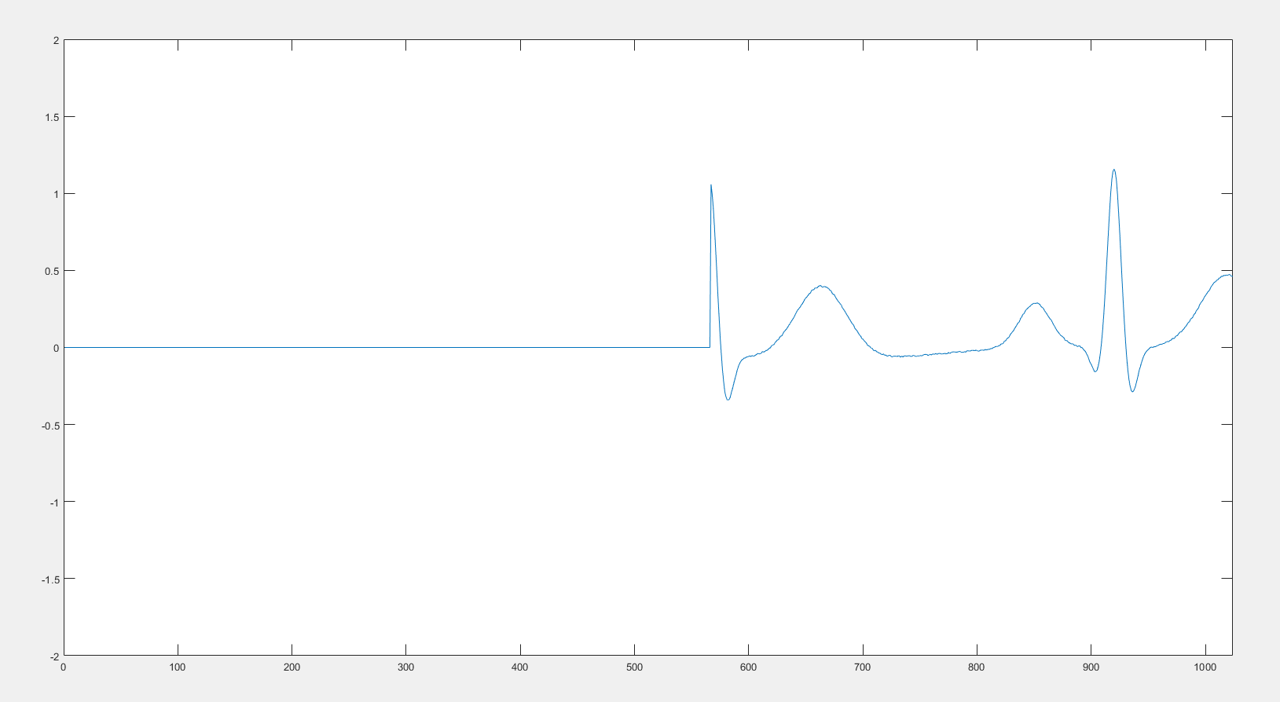
\includegraphics[width=1\columnwidth]{chapters/development/MATLAB/HALF_FILLED}
\end{figure}

\begin{figure}[!ht]
  \caption{Fixed length data buffer visualization fully filled}\label{fig:matlab_packet_test2}
  \centering
  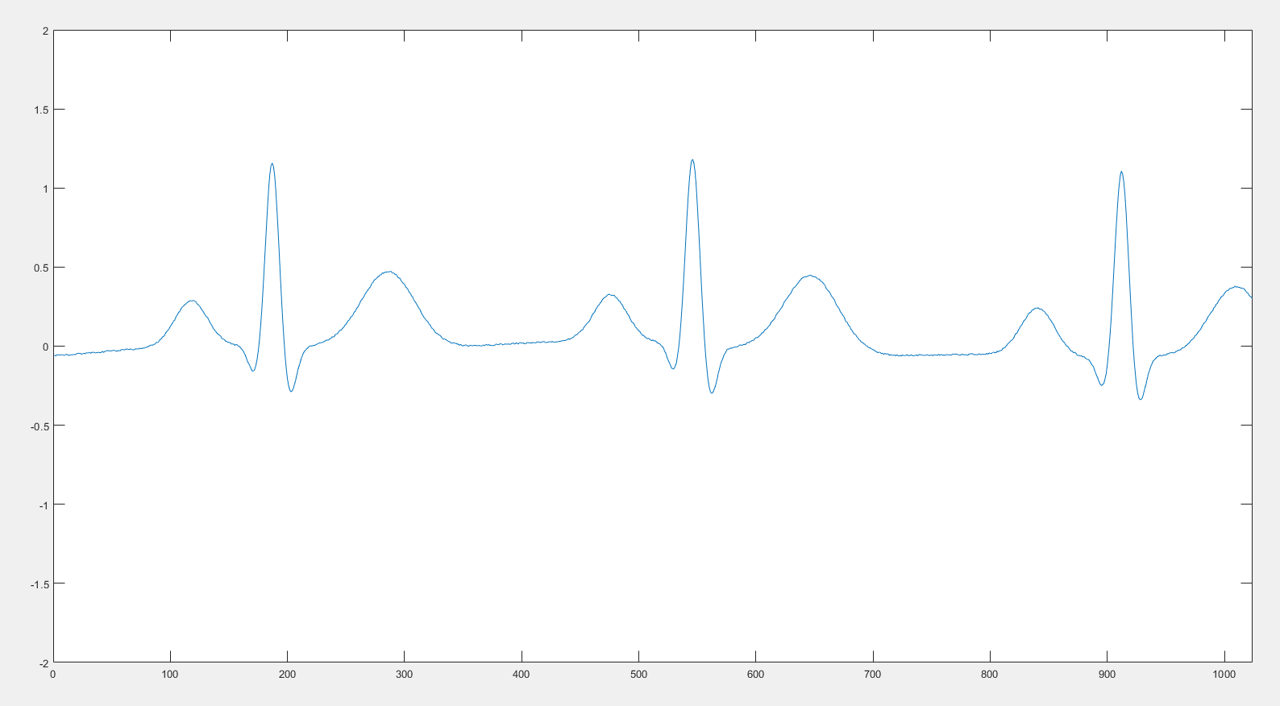
\includegraphics[width=1\columnwidth]{chapters/development/MATLAB/FULL_FILLED}
\end{figure}

\begin{lstlisting}[language=MATLAB,caption={MATLAB signal analaysis example}\label{code:matlab_analaysis}]
    %%% server side signal analaysis
    [peaks, locations, widths, prominances] = findpeaks(data);
    threshold = max(prominances) * .60;
    ecg_peak_locations = locations(prominances > threshold);

    peak_gap = zeros;
    for i = 2:length(ecg_peak_locations)
        peak_gap(i-1) = ecg_peak_locations(i) - ecg_peak_locations(i-1);
    end

    BPM = round(360 / mean(peak_gap) * 60, 0);
\end{lstlisting}

% TODO: WOULD BE GOOD TO HAVE SOME RESULT FROM THIS IN SOME CAPACITY
This code calcuates the BPM of the signal by measuring the gaps between the peaks of the ECG QRS signals.
It can be verified by comparing the measured BPM value with the given value from the dataset.
When the system is integrated, as long as the data length matches and the sensor data is accurate,
this same code will produce similar results.


\section{System Integration}
\subsection{Wireless Transmission}
With all the block of the system functional,
the first step of system integration is to establish communication between the off-body PC and on-body device.

On the on-body device, the ESP32 acts as the wireless bridge.
As this device requires a connection to WiFi for OTA updates, the wireless protocol that was choosen to be implemented was TCP/IP.
This is because the device already has a TCP/IP requirement and the only other choice for wireless communication was bluetooth, which does not have the range or speed that TCP/IP has.
The code for connecting the ESP32 to the off-body PC is shown in~\autoref{code:esp_tcpip_connect} and the corresponding MATLAB code is shown in~\autoref{code:matlab_tcpip}.

\begin{lstlisting}[language=C++,caption={ESP32 code for connecting to TCP/IP client}\label{code:esp_tcpip_connect}]
#include <WiFi.h>
#include <WiFiUdp.h>

WiFiClient client;

setup() {
  WiFi.mode(WIFI_STA);
  WiFi.begin(SSID, PASS);

  while (WiFi.waitForConnectResult() != WL_CONNECTED) {
    Serial.println(``Connection Failed! Rebooting...'');
    delay(5000);
    ESP.restart();
  }

  if (client.connect(SERVER_IP, SERVER_PORT)) { Serial.println('Connection success!'); }
  else { Serial.println('Connection failed!'); }
}

loop() {
  if (client.connected()) {
    client.write('T');
    client.write('E');
    client.write('S');
    client.write('T');
  }

  delay(500);
}
\end{lstlisting}

\lstinputlisting[language=MATLAB,caption={MATLAB TCPIP receive code}\label{code:matlab_tcpip}]{chapters/development/MATLAB/TCPIP_FIXED.m}

In order to get these devices to communicate, inbound and outbound rules need to be defined in the off-body PC firewall.
This is to allow connections on the specified port, since most PC ports are typically closed for security reasons.
The port settings can be seen in~\autoref{fig:firewall}.

\begin{figure}[!ht]
  \caption{TCP/IP firewall port settings}\label{fig:firewall}
  \centering
  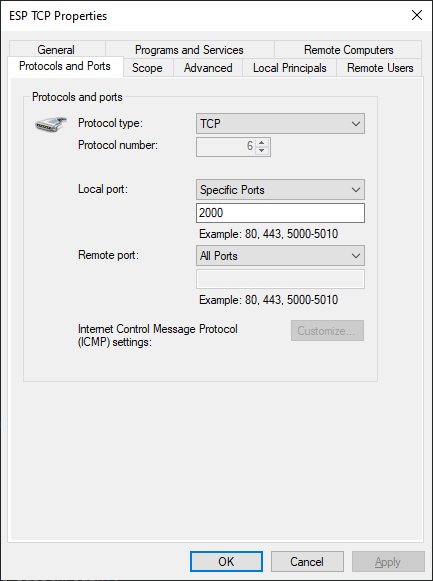
\includegraphics[width=1\columnwidth/2]{chapters/development/FIREWALL}
\end{figure}

With data being sent between the ESP32 and the off-body PC, the next device to connect is the PIC32 to the off-body PC.
Since the SPI communication between the PIC and the ESP has already been established,
the process buffer task can be updated to passthrough the received data to the off-body PC, this is shown in~\autoref{code:esp_tcpip_pic_passthrough}.
The other change to this SPI code is to add the client connection setup code from~\autoref{code:esp_tcpip_connect}.

\begin{lstlisting}[language=C++,caption={ESP32 code for connecting to TCP/IP client}\label{code:esp_tcpip_pic_passthrough}]
void task_process_buffer(void* pvParameters) {
  while (1) {
    ulTaskNotifyTake(pdTRUE, portMAX_DELAY);
    if (client.connected()) { client.write(buffer, slave.available()); }
    slave.pop();
    xTaskNotifyGive(task_handle_wait_spi);
  }
}
\end{lstlisting}

Then, the PIC can communicate with the off-body PC as shown in~\autoref{code:pic_offbody_pc_test}.

\begin{lstlisting}[language=C,caption={ESP32 code for connecting to TCP/IP client}\label{code:pic_offbody_pc_test}]
void init() {
  ESP32_init();
}

void run() {
  ESP32_SPI_write_byte('T');
  ESP32_SPI_write_byte('E');
  ESP32_SPI_write_byte('S');
  ESP32_SPI_write_byte('T');
  ESP32_SPI_write_byte('\n');

  delay(500);
}
\end{lstlisting}

\subsection{Base64}
Sending individual bytes between devices is now possible.
Currently, this only works as long as the value fits into a predetermined number of bytes.
Additionally, once the system is running with non-known values, there is no easy way to keep the data synchronized.
For instance, if a byte of data was lost, the received data would be in the incorrect place
and there would be no way of knowing.
This could be solved by sending a known byte sequence at the beginning of transmission.
However, there would be no differentiation between that byte sequence and any arbitrary data that may be being sent.
Another approach is to limit the character set so that specific byte values can correspond to `special' characters.
For example, the decimal value of 10, which corresponds to the newline character, could be used to mark the end of transmission.
That way, even if the transmitter and receiver become out of sync, the system has a way of recovering.
There are a number of character sets that have already been developed.

\begin{lstlisting}[language=C]
  void ESP32_SPI_write_array(uint8_t *array, size_t len) {
    for (size_t i = 0; i < len; i++) {
      ESP32_SPI_write_byte(array[i]);
    }
  }

  void write_packet(uint8_t* buf, size_t len) {
    uint8_t mod_table[] = {0, 2, 1};
    char encoding_table[] = {
      'A', 'B', 'C', 'D', 'E', 'F', 'G', 'H',
      'I', 'J', 'K', 'L', 'M', 'N', 'O', 'P',
      'Q', 'R', 'S', 'T', 'U', 'V', 'W', 'X',
      'Y', 'Z', 'a', 'b', 'c', 'd', 'e', 'f',
      'g', 'h', 'i', 'j', 'k', 'l', 'm', 'n',
      'o', 'p', 'q', 'r', 's', 't', 'u', 'v',
      'w', 'x', 'y', 'z', '0', '1', '2', '3',
      '4', '5', '6', '7', '8', '9', '+', '/'
    };

    size_t output_length = 4 * ((len + 2) / 3);
    char encoded_data[output_length];

    for (int i = 0, j = 0; i < len;) {
      uint32_t octet_a = i < len ? buf[i++] : 0;
      uint32_t octet_b = i < len ? buf[i++] : 0;
      uint32_t octet_c = i < len ? buf[i++] : 0;

      uint32_t triple = (octet_a << 0x10) + (octet_b << 0x08) + octet_c;

      encoded_data[j++] = encoding_table[(triple >> 3 * 6) & 0x3F];
      encoded_data[j++] = encoding_table[(triple >> 2 * 6) & 0x3F];
      encoded_data[j++] = encoding_table[(triple >> 1 * 6) & 0x3F];
      encoded_data[j++] = encoding_table[(triple >> 0 * 6) & 0x3F];
    }

    for (int i = 0; i < mod_table[len \% 3]; i++) {
      encoded_data[output_length - 1 - i] = '=';
    }

    ESP32_SPI_write_array(encoded_data, output_length);
    ESP32_SPI_write_byte('\n');
  }
\end{lstlisting}

\begin{lstlisting}[language=MATLAB]
base64 = readline(src);
decoded = transpose(matlab.net.base64decode(char(base64)));
\end{lstlisting}


\begin{lstlisting}[language=C]
void debug(const char *fmt, ...) {
    va_list args;
    char str[1024];

    va_start(args, fmt);
    vsprintf(str, fmt, args);
    va_end(args);

    write_packet(str, strlen(str));
}
\end{lstlisting}

\begin{lstlisting}[language=MATLAB]
y = char(decoded);
disp(y)
\end{lstlisting}

\begin{lstlisting}[language=C]
  int i = 0;

  void loop() {
    debug('Hello, World! \%u \n', i++);
    delay(500);
  }
\end{lstlisting}

\section{Testing and Validation}
What tests were performed and how that validates the system.
